% !TEX root = lectnote.tex
% !TEX spellcheck = en_GB-oed 

\chapter{Introduction}\label{cha:intro}





These lecture notes are based on the class material ``College Discrete Mathematics'' for students in the Foundation Semester year at University of Debrecen, Hungary. 
The lecture notes are intended to help the students understand and learn the course material, 
but they do not substitute participation and active work on the class. 

Discrete mathematics deals with the non-continuous mathematics.
This usually means finite mathematics, 
but properties of natural numbers are discussed, as well. 
The course sets the basis for future mathematical classes, 
and is essential to understand those later. 

In Chapter~\ref{cha:intro} we introduce basic mathematical concepts, 
such as sets, subsets, 
sums and products, 
the Euclidean algorithm and numeral systems. 
In Chapter~\ref{cha:counting} we show different counting arguments. 
We count the number of sequences, 
subsets, permutations, and anagrams. 
Then we consider the number of ordered subsets, 
the number of subsets of a given size. 
Finally, we count the number of possibilities to distribute money, 
and to take out some balls from an urn. 

In Chapter~\ref{cha:proof} we explain different basic mathematical proof methods, 
such as mathematical induction and
proof by contradiction. 
We show how one can prove theorems in a constructive way, 
or by using the pigeonhole principle. 
At the end of the chapter we use these proof techniques to bring the reader ``behind the curtains'' of a mathematical card trick. 

In Chapter~\ref{cha:Pascal} we consider Pascal's famous triangle built up from the binomial coefficients. 
We prove several identities related to the triangle, 
and use it to show the Binomial theorem. 
In Chapter~\ref{Recurrence sequences} recurrence sequences are discussed. 
We start by the famous Towers of Hanoi, 
then work our way up to more general recurrence sequences and to the explicit formulas determining them. 
Finally, in Chapter~\ref{cha:solutions} we give all solutions to the exercises occurring in the lecture notes. 


\section{Sets}\label{sec:sets}
In mathematics a set is a collection of objects that are called elements. Usually we denote sets by capital letters
and elements by small letters.
If $A$ is a set and $a$ is an element of $A$, then we write $a\in A$. If $a$ is not an element of $A$, then we write
$a\notin A$. Now we deal with the problem how to provide a set.
\begin{itemize}
\item \textbf{Sets given by enumeration.} If we have a set containing certain elements, then we enclose these elements
in braces. For example, if $A$ is a set containing 1, 2 and 3 we write $A=\halmaz{1,2,3}$. This notation is difficult to use
if the given set has large amount of elements. In this case we list only some (usually consecutive) elements such that
it is easy to see which are the remaining elements of the set. As an example let us assume that $B$ is a set containg
the integers between 1 and 1000. Here we write $B=\halmaz{1,2,3,\ldots,1000}$. If $C$ is the set containing the odd integers
between 1 and 99, then we have $C=\halmaz{1,3,5,\ldots,99}$. It is also possible to provide some families of sets, for example
$$D_1=\{1\},\quad D_k=\halmaz{1,3,\ldots,2k-1}.$$ 
In this case $D_k$ denotes the set containing the first $k$ positive odd integers.
\begin{center}
\begin{tabular}{|c|c|}
\hline
$k$ & $D_k$\\
\hline
1 & $\halmaz{1}$\\
\hline
2 & $\halmaz{1,3}$\\
\hline
3 & $\halmaz{1,3,5}$\\
\hline
4 & $\halmaz{1,3,5,7}$\\
\hline
\end{tabular}
\end{center}
\item \textbf{Standard sets.} There are certain frequently used sets which have their own symbols. These are the
set of natural numbers, the set of integers, the set of rational numbers, the set of real numbers and the set of
complex numbers.

$\mathbb{N}=\halmaz{1,2,3,\ldots}$, the set of natural numbers.

$\mathbb{Z}=\halmaz{\ldots,-2,-1,0,1,2,\ldots}$, the set of integers.

$\mathbb{Q}$, the set of rational numbers.

$\mathbb{R}$, the set of real numbers.

$\mathbb{C}$, the set of complex numbers.
\item \textbf{Set-builder notation.} It is also possible to define sets using the so-called set-builder notation.
As an example consider the set $D_3=\halmaz{1,3,5}$, we can define this set in many different ways, e.g.\
\begin{align*}
\halmaz{1,3,5}&=\halmazvonal{a}{(a-1)(a-3)(a-5)=0}, \\
\halmaz{1,3,5}&=\halmazvonal{a}{a=2k-1, k\in\halmaz{1,2,3}}, \\
\halmaz{1,3,5}&=\halmazvonal{a}{1\leq a\leq 5, \mbox{ and $a$ is odd}}.
\end{align*}
We can use semicolon instead of the vertical line, as well: 
\begin{align*}
\halmaz{1,3,5}&=\halmazpont{a}{(a-1)(a-3)(a-5)=0}, \\
\halmaz{1,3,5}&=\halmazpont{a}{a=2k-1, k\in\halmaz{1,2,3}}, \\
\halmaz{1,3,5}&=\halmazpont{a}{1\leq a\leq 5, \mbox{ and $a$ is odd}}.
\end{align*}
Let us define the set of even natural numbers: 
\[
\halmazvonal{2n}{n\in\mathbb{N}}.
\]
The set of rational numbers can be given as follows
\[
\halmazvonal{a/b}{a,b\in\mathbb{Z}, b\neq 0}.
\]
\end{itemize}
To study some basic properties of sets we give some definitions. First we introduce the concept of cardinality.
\begin{definition}
A set is called \emph{finite} if it has finite number of elements. If a set is not finite it is called \emph{infinite.}
\end{definition}
Now we consider cardinality of finite sets. The cardinality of infinite sets is more complicated and we will not 
discuss it.
\begin{definition}
Let $A$ be a finite set. The \emph{cardinality} of $A$ is the number of different elements of $A$. Notation: $|A|$.
\end{definition}
For example, the cardinality of $D_3$ is 3 and the cardinality of the set $\halmaz{1,2,3,6,7,8}$ is 6.
\begin{definition}
Let $A$ and $B$ be sets. The set $B$ is a \emph{subset} of $A$ if and only if every element of $B$ is an element of $A$.
Notation: $B\subseteq A$.
\end{definition}
There is a special set which is a subset of all sets, the so-called \emph{empty set.} As the name suggests it is the
set which has no element, that is, its cardinality is 0. The empty set is denoted by $\emptyset$.
\begin{definition}
If $B\subseteq A$ and $B\neq\emptyset, B\neq A$, then $B$ is a \emph{proper subset} of $A$.
\end{definition}
\begin{definition}
Let $A$ and $B$ be sets. The two sets are \emph{equal} if $A\subseteq B$ and $B\subseteq A$.
\end{definition}
Now we define some basic operations of sets.
\begin{definition}
Let $A$ and $B$ be sets. The \emph{intersection} of $A$ and $B$ is the set $\halmazvonal{x}{ x\in A \mbox{ and } x\in B}$. 
Notation: $A\cap B$.
\end{definition}
The so-called Venn diagrams are often useful in case of sets to understand the situation better. By shading
the appropriate region we illustrate the intersection of $A$ and $B$.
\begin{center}
\begin{venndiagram2sets}
\fillACapB
\end{venndiagram2sets}
\end{center}
Let $A=\halmaz{1,2,3,4,5}$ and $B=\halmaz{3,4,5,6,7}$. The intersection of these two sets is the set $A\cap B=\halmaz{3,4,5}$.
\begin{definition}
Let $A$ and $B$ be sets. The \emph{union} of $A$ and $B$ is the set $\halmazvonal{x}{x\in A \mbox{ or } x\in B}$.
Notation: $A\cup B$.
\end{definition}
The corresponding Venn diagram is as follows.
\begin{center}
\begin{venndiagram2sets}
\fillA\fillB
\end{venndiagram2sets}
\end{center}
Let $A=\halmaz{1,2,3,4,5}$ and $B=\halmaz{3,4,5,6,7}$. The union of these two sets is the set $A\cup B=\halmaz{1,2,3,4,5,6,7}$.
It is easy to see that the following properties hold $A\cap B=B\cap A$ and $A\cup B=B\cup A$. It is not true for
the difference of two sets.
\begin{definition}
Let $A$ and $B$ be sets. The \emph{difference} of $A$ and $B$ is the set $\halmazvonal{x}{ | x\in A \mbox{ and } x\notin B}$. Notation: $A\setminus B$.
\end{definition}
The Venn diagram of $A\setminus B:$
\begin{center}
\begin{venndiagram2sets}
\fillOnlyA
\end{venndiagram2sets}
\end{center}
To see the difference between $A\setminus B$ and $B\setminus A$ we draw 
the Venn diagram of $B\setminus A$ as well:
\begin{center}
\begin{venndiagram2sets}
\fillOnlyB
\end{venndiagram2sets}
\end{center}
Again, let $A=\halmaz{1,2,3,4,5}$ and $B=\halmaz{3,4,5,6,7}$. Now we have that
\begin{align*}
A\setminus B &=\halmaz{1,2},\\
B\setminus A &=\halmaz{6,7}.
\end{align*}
Now we introduce the symmetric difference of sets.
\begin{definition}
Let $A$ and $B$ be sets. The \emph{symmetric difference} of $A$ and $B$ is the set $(A\cup B)\setminus(A\cap B)$. Notation: $A\triangle B$.
\end{definition}
The Venn diagram of the symmetric difference of $A$ and $B:$
\begin{center}
\begin{venndiagram2sets}
\fillANotB\fillBNotA
\end{venndiagram2sets}
\end{center}
We give an example using sets $A=\halmaz{1,2,3,4,5}$ and $B=\halmaz{3,4,5,6,7}$. We obtain that
$$
A\triangle B=\halmaz{1,2,6,7}.
$$
Finally, we define the complement of a set.
\begin{definition}
Let $U$ be a set (called the universe) and $A$ is a subset of $U.$
The complement of $A$ consists of elements of $U$ which do not belong to $A.$
Notation: $\overline{A}.$
\end{definition}
The corresponding Venn diagram is as follows.
\begin{center}
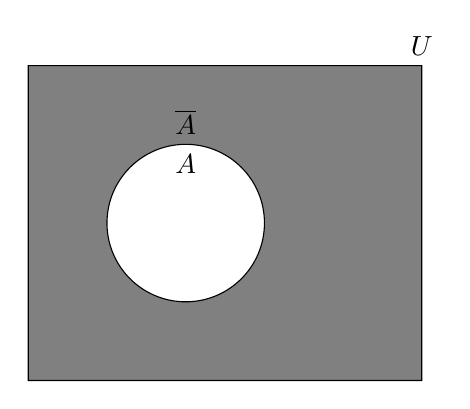
\begin{tikzpicture}
\filldraw[fill=gray] (-2,-2) rectangle (3,2);
\scope % A \cap B
\clip (0,0) circle (1);
\fill[white] (0,0) circle (1);
\endscope
% outline
\draw (0,0) circle (1) (0,1) node [text=black,below] {$A$}
      (0,0) circle (1) (0,1) node [text=black,above] {$\overline{A}$}
      (-2,-2) rectangle (3,2) node [text=black,above] {$U$};
      %(1,0) circle (1);
\end{tikzpicture}
\end{center}
As an example consider the sets $U=\{1,2,3,4,5,6\}$ and $A=\{1,3,5\}.$ The complement of $A$ is
the set $\{2,4,6\}.$
\begin{exercise}\label{intro-ex-1}
Let $A=\halmaz{3,4,6,7,8},B=\halmaz{2,4,5,6,8}$ and $C=\halmaz{1,2,4,5,8}$. 
What are the elements of the set $(A\setminus B)\cup(C\cap B)$?
\end{exercise}
\begin{exercise}\label{intro-ex-2}
Let $A=\halmaz{1,3,4,6,7},B=\halmaz{2,4,5,6,8}$ and $C=\halmaz{1,3,4,5,8}$. 
What are the elements of the set $(A\cap B)\setminus(C\cap B)$?
\end{exercise}
\begin{exercise}\label{intro-ex-3}
Let $A=\halmaz{1,3,4,6,7},B=\halmaz{2,4,6,8}$ and $C=\halmaz{1,3,4,8}$. 
What are the elements of the set $(A\setminus B)\cup(C\setminus B)$?
\end{exercise}
\begin{exercise}\label{intro-ex-4}
List all elements of the following sets:

(a) $\halmazvonal{3k+1}{k\in\halmaz{2,3,4}}$,

(b) $\halmazvonal{k^2}{ k\in\halmaz{-1,0,1,2}}$,

(c) $\halmazvonal{u-v}{u\in\halmaz{3,4,5}, v\in\halmaz{1,2}}$. 
\end{exercise}
\begin{exercise}\label{intro-ex-5}
Describe the following sets using set-builder notation.

(a) $\halmaz{2,4,6,8,10}$,

(b) $\halmaz{1,4,9,16,25}$,

(c) $\halmaz{1,\frac{1}{2},\frac{1}{4},\ldots, \frac{1}{2^k}, \ldots}$,

(d) the set of rational numbers between 1 and 2.
\end{exercise}
\begin{exercise}\label{intro-ex-6}
Draw a Venn diagram for the following sets:

(a) $(A\cap B)\cup C$,

(b) $(A\setminus B)\cup(A\setminus C)$,

(c) $(A\cup B)\cap C$,

(d) $(A\cap B)\cup(B\cap C)\cup(A\cap C)$,

(e) $\left((A\cap B)\setminus C\right)\cup \left((A\cap C)\setminus B\right)\cup \left((B\cap C)\setminus A\right)$,

(f) $(A\setminus B)\cup(B\setminus C)\cup(C\setminus A)$.
\end{exercise}
\begin{exercise}\label{intro-ex-7}
Provide three sets $A,B$ and $C$ which satisfy the following cardinality conditions
$$
|A\cap B\cap C|=2,
$$
$$
|A\cap B|=|A\cap C|=|B\cap C|=2,
$$
$$
|A|=|B|=|C|=4.
$$
\end{exercise}
\begin{exercise}\label{intro-ex-8}
Provide three sets $A,B$ and $C$ which satisfy the following cardinality conditions
$$
|A\cap B\cap C|=2,
$$
$$
|A\cap B|=2,\quad |A\cap C|=2,\quad |B\cap C|=3,
$$
$$
|A|=4,\quad |B|=5,\quad |C|=6.
$$
\end{exercise}

\section{Sums and products}\label{sec:sumsproducts}
In this section we introduce summation notation and product notation which we will use later on.
The special symbol $\sum$ is used to denote sums. Let us consider an example
$$
\sum_{k=1}^5 k=1+2+3+4+5.
$$
In a more general form
$$
\sum_{k=m}^n k=m+(m+1)+\ldots+(n-1)+n.
$$
Here $m$ is the lower bound of summation and $n$ is the upper bound of summation.
There are some other possibilities to express the above sum, e.g.\
\begin{align*}
&\sum_{m\leq k\leq n}k,\\
&\sum_{k\in S}k, \mbox{ where }S=\halmaz{m,m+1,\ldots,n}.
\end{align*}
It is important to note that the variable used in the summation is arbitrary. That is, 
the values of the following summations are equal:
$$
\sum_{k=1}^3 k^2=1^2+2^2+3^2=14
$$
and
$$
\sum_{m=1}^3 m^2=1^2+2^2+3^2=14.
$$
Now we write out explicitly some other summations:

(a) $$\sum_{i=2}^6 (2-i)=(2-2)+(3-2)+(4-2)+(5-2)+(6-2)=10,$$

(b) $$\sum_{j=3}^5 2^{j-2}=2^{3-2}+2^{4-2}+2^{5-2}=14,$$

(c) $$\sum_{1\leq i,j\leq 2} ij= (1\cdot 1)+(1\cdot 2)+(2\cdot 1)+(2\cdot 2)=9.$$

Now we deal with products of mathematical expressions. The symbol used in this case is $\prod$.
Product notation is very similar to summation notation so it is straightforward to learn to use.
The first example in case of summation notation was 
$$
\sum_{k=1}^5 k=1+2+3+4+5.
$$
If we change the $\sum$ symbol to $\prod$, then we obtain
$$
\prod_{k=1}^5 k=1\cdot 2\cdot 3\cdot 4\cdot 5.
$$
Let us consider the product of integers between $m$ and $n$, where $m<n$. We can write it in 
product notation in different forms:
\begin{align*}
&\prod_{k=m}^n k,\\
&\prod_{m\leq k\leq n}k,\\
&\prod_{k\in S}k, \mbox{ where }S=\halmaz{m,m+1,\ldots,n}.
\end{align*}
It may happen that the sum or product should be evaluated on the empty set. 
By definition, in such situations the sum is always 0 and the product is always 1, 
e.g.\
\begin{align*}
\sum_{k \in \emptyset} k &= 0, \\
\prod_{k \in \emptyset} k &= 1. 
\end{align*}
If $S$ and $T$ be two disjoint sets, then 
\begin{align*}
\sum_{k \in S} k + \sum_{k \in T} k = \sum_{k \in S \cup T} k, \\
\prod_{k \in S} k \cdot \prod_{k \in T} k = \prod_{k \in S \cup T} k. 
\end{align*}
Note, that this is true even if $S$ or $T$ is the empty set. 
(This is the main reason we define the empty sum to be 0 and the empty product to be 1.)

There is a special notation for the product of positive integers up to $n$, 
that is, when we multiply the elements of 
\[
S_n = \halmazvonal{k}{k \text{ is a positive integer}, k\leq n} = \halmaz{1, 2, \dots , n}. 
\]
The product of the elements of $S_n$ is called \emph{$n$ factorial} and denoted by $n!$, 
that is, 
\[
n! = \prod_{k \in S_n} k = \prod_{k=1}^n k = 1 \cdot 2 \cdot \dots \cdot (n-1) \cdot n. 
\]
We even define $0!$, 
that is, the products of elements of $S_0$: 
\[
0! = \prod_{k \in S_0} k = \prod_{k \in \emptyset} k = 1.
\]
Factorials are always computed before any other operation. 
For example
\begin{align*}
2+3! &= 2 + 1\cdot 2 \cdot 3 = 2 + 6 = 8, \\
(2+3)! &= 5! = 1\cdot 2 \cdot 3 \cdot 4 \cdot 5 = 120. 
\end{align*}



\begin{exercise}\label{intro-ex-9}
Expand the following sums.

(a) $\sum_{i=4}^7 i$,

(b) $\sum_{i=1}^5 (i^2-i)$,

(c) $\sum_{i=1}^4 10^i$,

(d) $\sum_{2\leq i\leq 5} \frac{1}{2^i}$,

(e) $\sum_{i\in S} (-1)^i$, where $S=\halmaz{2,3,5,8}$.
\end{exercise}

\begin{exercise}\label{intro-ex-10}
Write the following expressions in summation notation.

(a) $2+4+6+8+10$,

(b) $1+4+7+10$,

(c) $\frac{1}{4}+\frac{1}{2}+1+2+4$,

(d) $\frac{1}{4}-\frac{1}{2}+1-2+4$.
\end{exercise}

\begin{exercise}\label{intro-ex-11}
Expand the following products.

(a) $\prod_{i=-4}^{-1} i$,

(b) $\prod_{i=1}^4 (i^2)$,

(c) $\prod_{i=1}^3 2^i$,

(d) $\prod_{-2\leq i\leq 3} \frac{1}{2^i}$,

(e) $\prod_{i\in S} (-1)^i$, where $S=\halmaz{2,4,6,7}$. 
\end{exercise}

\begin{exercise}\label{intro-ex-12}
Write the following expressions in product notation.

(a) $1\cdot 3\cdot 5\cdot 7$,

(b) $(-1)\cdot 2\cdot 5\cdot 8$,

(c) $\frac{1}{9}\cdot\frac{1}{3}\cdot 1\cdot 3\cdot 9$.
\end{exercise}

\begin{exercise}\label{ex:factorial1}
Compute the values of $n!$ for every $n \in \halmaz{0, 1, 2, 3, 4, 5, 6, 7, 8}$. 
\end{exercise}

\begin{exercise}\label{ex:factorial2}
Compute the values of 
\begin{align*}
& 5+3! \\
& (5+3)! \\
& 4-2\cdot 3! \\
& (4-2)\cdot 3! \\
& 4 - (2 \cdot 3)! \\
& 3 \cdot 2! \\
& (3 \cdot 2)! \\
& 4 \cdot 3! \\
& 4! \cdot 5. 
\end{align*}
\end{exercise}

\begin{exercise}\label{ex:factorial3}
Prove that $n! = n \cdot (n-1)!$ for every positive integer $n$. 
Note, that it is even true for $n=1$, 
which is one of the reasons we define $0!$ to be equal to 1. 
\end{exercise}





\section{The Euclidean algorithm}\label{Euc}
In this section we introduce the so-called Division algorithm, we define the greatest common divisor of given integers and we consider
the Euclidean algorithm, which is one of the oldest mathematical algorithms.

{\bf Division algorithm.} Given two integers $a$ and $b$ such that $b>0$. There exist unique integers $q$ and $r$ for which 
$$
a=qb+r,\quad 0\leq r<b.
$$
Here $q$ is called \emph{quotient} and $r$ is called \emph{remainder.}
There is a special case, when the Division algorithm yields $r=0$. In such a situation $a=qb$ for some $q$.
\begin{definition}
We say that $b$ \emph{divides} $a$ ($b$ is a \emph{divisor} of $a$ or $a$ is a \emph{multiple} of $b$) if there exists $q$ such that $a=qb$.
Notation: $b\mid a$.
\end{definition}
How to find an appropriate $q$ and $r$? Let us assume that we have two positive integers $a$ and $b$. We start with $q=0$ and $r=a$.
Clearly $a=0\cdot b+a$. If $a<b$, then we are done, otherwise $a-b\geq 0$. So we write $a=1\cdot b+(a-b)$. We check if $a-b<b$. If this is the case
then we have found $q$ and $r$, otherwise we have $a-2b\geq 0$ and $a=2\cdot b+(a-2b)$. We stop when we have $a-kb<b$ for some $k$. For example, let 
$a=76$ and $b=7:$
\begin{center}
\begin{tabular}{|c|c|}
\hline
$k$ & $a-kb$\\
\hline
0 & 76\\
\hline
1 & 69\\
\hline
2 & 62\\
\hline
3 & 55\\
\hline
4 & 48\\
\hline
5 & 41\\
\hline
6 & 34\\
\hline
7 & 27\\
\hline
8 & 20\\
\hline
9 & 13\\
\hline
10 & 6\\
\hline
\end{tabular}
\end{center}
that is, we obtain that $76=10\cdot 7+6$ and $0\leq 6<7$.
\begin{definition}
Let $a,b\in\mathbb{Z}$. A positive integer $d$ is called a \emph{common divisor} of $a$ and $b$, if $d$ divides $a$
and $d$ divides $b$. The largest possible such integer is called the \emph{greatest common divisor} of $a$ and $b$. 
Notation: $\gcd(a,b)$.
\end{definition}

{\bf The Euclidean algorithm.} Now we study a method to determine $\gcd(a,b)$ of given positive integers $a$ and $b$.
The method also provides solution of the linear Diophantine equation
$$
ax+by=\gcd(a,b).
$$
If we apply the Division algorithm to $a,b,a>b$, then we have
$$
a=qb+r,\quad 0\leq r<b.
$$
If $d$ is a common divisor of $a$ and $b$, then $d$ divides $r=a-qb$ as well. That is the basic idea of the algorithm.
The Euclidean algorithm works as follows. First we apply the Division algorithm for $a$ and $b$ to obtain a quotient $q_1$ and a remainder $r_1$.
Then we apply the Division algorithm for $b$ and $r_1$ to get a new quotient $q_2$ and a new remainder $r_2$. We continue, we divide
$r_1$ by $r_2$ to obtain $q_3$ and $r_3$. We stop if we obtain a zero remainder. Since the procedure produces a decreasing sequence of non-negative integers
so must eventually terminate by descent.
The last non-zero remainder is the greatest common divisor
of $a$ and $b$.

As an example we compute $\gcd(553,161)$. We write the computations in the following way:
\begin{align*}
553&=3\cdot 161+70\quad q_1=3, r_1=70\\
161&=2\cdot 70+21\quad q_2=2, r_2=21\\
70&=3\cdot 21+7\quad q_3=3, r_3=7\\
21&=3\cdot 7+0\quad q_4=3, r_4=0.
\end{align*}
That is, the last non-zero remainder is 7, so $\gcd(553,161)=7$.
If we would like to express 7 as $553x+161y$ for some $x,y\in\mathbb{Z}$, we can do it by working backwards
\begin{align*}
7&=70-3\cdot 21\\
 &=70-3\cdot (161-2\cdot 70)=-3\cdot 161+7\cdot 70\\
 &=-3\cdot 161+7 \cdot (553-3\cdot 161)=7\cdot 553-24\cdot 161.
\end{align*}
It follows that $x=7$ and $y=-24$.

\begin{exercise}\label{intro-ex-13}
Use the Euclidean algorithm to find $\gcd(a,b)$ and compute integers $x$ and $y$ for which
$$
ax+by=\gcd(a,b):
$$

(a) $a=678, b=567$,

(b) $a=803, b=319$,

(c) $a=2701, b=2257$,

(d) $a=3397, b=1849$.
\end{exercise}

\section{Numeral systems}\label{sec:numeralsystem}

In this Section we learn about the different numeral systems. 
In everyday life we use base 10. 
That is, 
when we talk about numbers, 
we use the base 10 notation. 

Let us consider counting. 
Imagine Robinson Crusoe spending his days on an uninhabited island, 
and he counts all the days by carving a vertical line every day into a rock. 
He was raised using the base 10 numbers, 
thus after reaching 9 lines, 
he crosses them on the tenth day (thus marking them as ten). 
That way he groups together every ten days. 
Then, when he reaches ten of such groups, 
then he carves a big box around them. 
That is how he indicates hundreds. 
Then he circles around every ten boxes, 
indicating thousands, etc. 
Then, reaching ten circles on one rock he would look for a new rock to carve days into. 

Assume Robinson had arrived at the island 1st May 1817, 
and was rescued on 30th April 1850. 
How would his stones look like, 
after so much time?
He spent 33 years on the island, 
that is, $33 \cdot 365 = 12045$ days, not counting leap years. 
The leap years are 1820, 1824, 1828, 1832, 1836, 1840, 1844, 1848, 
that is, he spent $12053$ days altogether on the island. 
That means one of the ten thousands, 
two of the thousands, zero of hundreds, five of tens and three of ones. 
That is, he would have one rock completely full with ten circles, 
ten boxes in each circle, 
and ten of the ten lines crossed in each box. 
Then on his second rock he would have two full circles, 
and next to them he would have five of the ten crossed lines and three separate lines. 

Robinson is basically writing the numbers in base 10 by grouping every ten together. 
This is what we do, as well, 
except maybe in a bit more abstract and automatic way. 
When we think about the number 12053, 
we automatically give the meaning to the positions with the appropriate powers of 10: 
\begin{align*}
12053 &= 1 \cdot 10~000 + 2 \cdot 1~000 + 0 \cdot 100 + 5 \cdot 10 + 3 \cdot 1 = \\
&= 1 \cdot 10^4 + 2 \cdot 10^3 + 0 \cdot 10^2 + 5 \cdot 10^1 + 3 \cdot 10^0. 
\end{align*}

By writing the digits next to each other we indicate their value by their positioning. 
The value of the rightmost digit is $1 = 10^0$, 
then going from right to left the value increases by a factor of 10. 
That is, the value of the second rightmost digit is $10^1$, 
the digit left from it is $10^2$, etc. 
We have ten digits altogether (0, 1, 2, 3, 4, 5, 6, 7, 8, 9), 
because every tens will be grouped together by this positioning. 

All other numeral systems are based on the same idea. 
Considering for example base 2 (the \emph{binary system}), 
we will only need two digits: 0 and 1, 
because every twos will be grouped together. 
The values of the digits from right to left will be the two powers in increasing order, 
that is, 1, 2, 4, 8, 16, 32, 64, etc. 
We indicate by the number 2 in the lower right corner of the number that the base is 2. 
For example 
\[
101011_{2} = 1 \cdot 2^5 + 0 \cdot 2^4 + 1 \cdot 2^3 + 0 \cdot 2^2 + 1 \cdot 2^1 + 1 \cdot 2^0 = 32 + 8 + 2 + 1 = 43_{10}.
\]
Numbers are almost exclusively represented in their binary form in Computer Science. 

Another typical example from Computer Science could be the \emph{octal system,} 
i.e.\ base 8 (1 byte equals to 8 bits). 
Then there are eight digits (0, 1, 2, 3, 4, 5, 6, 7), 
and the values of the digits from right to left are the increasing powers of 8. 
Similarly, in Computer Science, base 16 \emph{(hexadecimal number system)} is used. 
Here, the values of the digits from right to left are the increasing powers of 16, 
and we need 16 digits. 
That is, we need separate digits for the digits corresponding to 10, 11, 12, 13, 14 and 15. 
By convention, we denote these digits by the first six letters of the alphabet: 
\begin{align*}
A_{16} &= 10_{10}, & B_{16} &= 11_{10} & C_{16} = 12_{10}, \\
D_{16} &= 13_{10}, & E_{14} &= 14_{10} & F_{16} = 15_{10}. 
\end{align*}

At first, it might look strange to use digits for the number ten, eleven or twelve. 
This is actually not so surprising if we think about some historical number systems. 
Counting months, or looking at the clock we use base 12 numeral system. 
Until 1971 British people used base 12 for money exchange (12 pennies were worth 1 shilling). 
Moreover, 
in the English language eleven and twelve have different names, 
they are not generated as all the others between 10 and 20, 
indicating that they may have been distinguished as extra digits. 

Generally, 
in base $n$ we need $n$ digits, running from 0 to $(n-1)$. 
We will write numbers in positional system, as above. 
The values of the digits are the powers of $n$ going from right to left. 
That is, the rightmost digit has value $n^0 = 1$, 
the second rightmost digit has value $n^1 = n$, 
the digit left to it has value $n^2$, etc. 
Thus, the number $a_ta_{t-1} \dots a_2a_1a_0$ in base $n$ 
(where $0\leq a_k \leq n-1$ for every $0\leq k\leq t$) 
represents the number
\[
(a_ta_{t-1} \dots a_2a_1a_0)_{n} = \sum_{k=0}^t a_k \cdot n^k = a_t \cdot n^t + a_{t-1} \cdot n^{t-1} + \dots + a_2 \cdot n^2 + a_1 \cdot n^1 + a_0 \cdot n^0. 
\]

Now, the question is how to write numbers into different numeral systems. 
First of all, to write numbers from a numeral system into base 10
we basically calculate the values of the digits using the positional systems, 
and sum the results: 
\begin{align*}
10101_2 &= 1 \cdot 2^4 + 0 \cdot 2^3 +1 \cdot 2^2 + 0 \cdot 2^1 + 1 \cdot 2^0 = 16 + 4 + 1 = 21_{10} \\
1212_3 &= 1 \cdot 3^3 + 2 \cdot 3^2 + 1 \cdot 3^1 + 2 \cdot 3^0 = 27 + 18 + 3 + 2 = 50_{10} \\
372_8 &= 3 \cdot 8^2 + 7 \cdot 8^1 + 2 \cdot 8^0 = 192 + 56 + 2 = 250_{10} \\
AFE_{16} &= 10 \cdot 16^2 + 15 \cdot 16^1 + 14 \cdot 16^0 = 2560 + 240 + 14 = 2814_{10}. 
\end{align*}
Another method is to repeatedly multiply by the base and add the next digit. 
For example: 
\begin{align*}
10101_2 &= (((1 \cdot 2 + 0 ) \cdot 2 + 1)\cdot 2 + 0) \cdot 2 + 1  \\
& ((2 \cdot 2 + 1)\cdot 2 + 0) \cdot 2 + 1 = (5 \cdot 2 + 0) \cdot 2 + 1=  21_{10} \\
1212_3 &= ((1 \cdot 3 + 2) \cdot 3 + 1) \cdot 3 + 2 \\
&= (5 \cdot 3 + 1)\cdot 3 + 2 = 16 \cdot 3 + 2 = 50_{10} \\
372_8 &= (3 \cdot 8 + 7) \cdot 8 + 2 = 31 \cdot 8 + 2 = 250_{10} \\
AFE_{16} &= (10 \cdot 16 + 15) \cdot 16 + 14 = 175 \cdot 16 + 14 = 2814_{10}. 
\end{align*}

The other direction is to find a base $n$ representation of a decimal number. 
Again, it can be done in two different ways. 
The first is that we check the highest $n$-power which is not greater than our number, 
execute division algorithm with this $n$-power, 
and repeat the process for the remainder, 
until the remainder is 0. 
For example, write $250_{10}$ in base 8. 
The 8-powers are (in increasing order) 1, 8, 64, 512, 
the last one is already greater than 250. 
Thus we execute the division algorithm with 64: 
$250 = 3 \cdot 64 + 58$. 
Now, 8 is not greater than 58, thus we execute the division algorithm by 8: 
$58 = 7 \cdot 8 + 2$. 
Finally, 
1 is the highest 8-power not greater than 2, 
and after the division algorithm we obtain $2 = 2 \cdot 1 +0$. 
Thus 
\[
250_{10} = 3 \cdot 64 + 7 \cdot 8 + 2 \cdot 1 = 3 \cdot 8^2 + 7 \cdot 8^1 + 2 \cdot 8^0 = 372_8. 
\]

\begin{exercise}\label{ex:numsyst1}
Write $21_{10}$ in base 2, 
$50_{10}$ in base 3, 
$2814_{10}$ in base 16 using the method explained above. 
\end{exercise}

The other method is to execute the division algorithm repeatedly on the quotients until the quotient is not 0, 
and then the number will consist of the remainders \emph{backwards}. 
For example, if we want to rewrite $2814_{10}$ into base 16, then 
\begin{align*}
2814 &= 175 \cdot 16 + 14, \\
175 &= 10 \cdot 16 + 15, \\
10 &= 0 \cdot 16 + 10. 
\end{align*}
The remainders backwards are $10=A$, $15=F$, $14=E$, thus 
\[
2814_{10} = AFE_{16}.
\]
\begin{exercise}\label{ex:numsyst2}
Write $21_{10}$ in base 2, 
$50_{10}$ in base 3, 
$250_{10}$ in base 8 using the division algorithm. 
\end{exercise}

How would we write a number of an arbitrary base into another (arbitrary) base? 
One method could be that we simply rewrite it first into base 10, 
then write it into the other system. 
For example, if we need to write $372_8$ into base 3, we can do the following. 
Rewrite $372_8$ first into base 10: 
\[
372_8 = 3 \cdot 8^2 + 7 \cdot 8^1 + 2 \cdot 8^0 = 192 + 56 + 2 = 250_{10}. 
\]
Now, rewrite $250_{10}$ into base 3:
\begin{align*}
250 &= 83 \cdot 3 + 1, \\
83 &= 27 \cdot 3 + 2, \\
27 &= 9 \cdot 3 + 0, \\
9 &= 3 \cdot 3 + 0, \\
3 &= 1 \cdot 3 + 0, \\
1 &= 0 \cdot 3 + 1. 
\end{align*}
The remainders backwards are 1, 0, 0, 0, 2, 1, thus 
\[
372_8 = 250_{10} = 100021_{3}. 
\]

Finally, we mention that some rewriting can be done much quicker if one base is a full power of another. 
For example, $8=2^3$, and then every base 8 digit can be rewritten easily to three base 2 digits: 
\begin{align*}
0_8 &= 000_2, & 1_8 &= 001_2, \\
2_8 &= 010_2, & 3_8 &= 011_2, \\
4_8 &= 100_2, & 5_8 &= 101_2, \\
6_8 &= 110_2, & 7_8 &= 111_2. 
\end{align*}
Going from right to left, 
every three base 2 digits can be easily rewritten into base 8, as well. 
Thus, it is easy to rewrite $372_8$ into base 2 or $10101_2$ into base 8: 
\begin{align*}
372_8 &= 011~111~010_2 = 11111010_2, \\
10101_2 &= 010~101_2 = 25_8. 
\end{align*}

Similarly, 
as $16 = 2^4$, 
every base 16 digit can be rewritten easily to four base 2 digits: 
\begin{align*}
0_{16} &= 0000_2, & 1_{16} &= 0001_2, \\
2_{16} &= 0010_2, & 3_{16} &= 0011_2, \\
4_{16} &= 0100_2, & 5_{16} &= 0101_2, \\
6_{16} &= 0110_2, & 7_{16} &= 0111_2, \\
8_{16} &= 1000_2, & 9_{16} &= 1001_2, \\
A_{16} &= 1010_2, & B_{16} &= 1011_2, \\
C_{16} &= 1100_2, & D_{16} &= 1101_2, \\
E_{16} &= 1110_2, & F_{16} &= 1111_2. 
\end{align*}
Going from right to left, 
every four base 2 digits can be easily rewritten into base 16, as well. 
Thus, it is easy to rewrite $AFE_{16}$ into base 2 or $10101_2$ into base 16: 
\begin{align*}
AFE_{16} &= 1010~1111~1110_2 = 101011111110_2, \\
10101_2 &= 0001~0101_2 = 15_{16}. 
\end{align*}

We have to stress, though, that this method only works \emph{if one base is a full power of the other}. 
Finally, base 8 numbers can be easily changed to base 16 (and vice versa) by first changing them to base 2, 
and then into the other base: 

\begin{align*}
372_8 &= 011~111~010_2 = 11111010_2 = 1111~1010_2 = FA_{16}, \\
AFE_{16} &= 1010~1111~1110_2 = 101011111110_2 = 101~011~111~110_2 = 5376_8. 
\end{align*}

\begin{exercise}\label{ex:numsyst3}
\begin{enumerate}
\item[(a)]
Write the following numbers into base 10: 
$111001101_2$, $1010101_2$, $11111_2$, $10110_2$, $101010101_2$, $10001000_2$, $1010111_2$, $111101_2$, 
$21102_3$, $1234_5$, $1234_7$, 
$1234_8$, $777_8$, $345_8$, $2012_8$, $4565_8$, $1123_8$, $666_8$, $741_8$, 
$CAB_{16}$, $BEE_{16}$, $EEE_{16}$, $4D4_{16}$, $ABC_{16}$, $9B5_{16}$, $DDD_{16}$, $3F2_{16}$. 

\item[(b)]
Write the following decimal numbers into base 2, 3, 5, 7, 8, 9, 16: \\
$64_{10}$, $50_{10}$, $16_{10}$, $100_{10}$, $2012_{10}$, $200_{10}$, $151_{10}$, $48_{10}$, $99_{10}$, $999_{10}$. 

\item[(c)]
Rewrite the given numbers into the particular numeral system: 
\begin{align*}
1121_3 &= \dots \dots \, _2, \\
4312_5 &= \dots \dots \, _7, \\
654_8 &= \dots \dots \, _9, \\
AD2_{16} &= \dots \dots \, _7, \\
543_8 &= \dots \dots \, _3, \\
543_9 &= \dots \dots \, _3. 
\end{align*}

\item[(d)]
Write the following numbers into base 2 and base 16: 
$777_8$, $345_8$, $2012_8$, $456_8$, $235_8$, $147_8$, $741_8$, 
$CAB_{16}$, $BEE_{16}$, $EEE_{16}$, $4D3_{16}$, $ABC_{16}$, $FEE_{16}$, $9B5_{16}$, $3F2_{16}$. 
\end{enumerate}
\end{exercise}






%We start counting by 1, 2, 3, 4, 5, 6, 7, 8, 9. 
%Then after 9 comes 10, which is a two-digit number, 
%because we grouped together a ten, and there are no ones. 
%Then we continue with 11, 
%where there are 1 of the tens and 1 of the ones. 
%Then comes 12, 
%where we have 1 of the tens and 2 of the ones. 
%Then comes 13, 14, 15, 16, 17, 18, 19. 
%After 19 comes 20, where we have another ten to group together,. 



























